\documentclass[tikz]{standalone}
\usepackage{amsmath}
\usepackage{xcolor}
\usepackage{tikz}
\tikzstyle{format} = [rectangle, draw, fill = blue!20]
\usetikzlibrary{er,positioning}

\begin{document}
    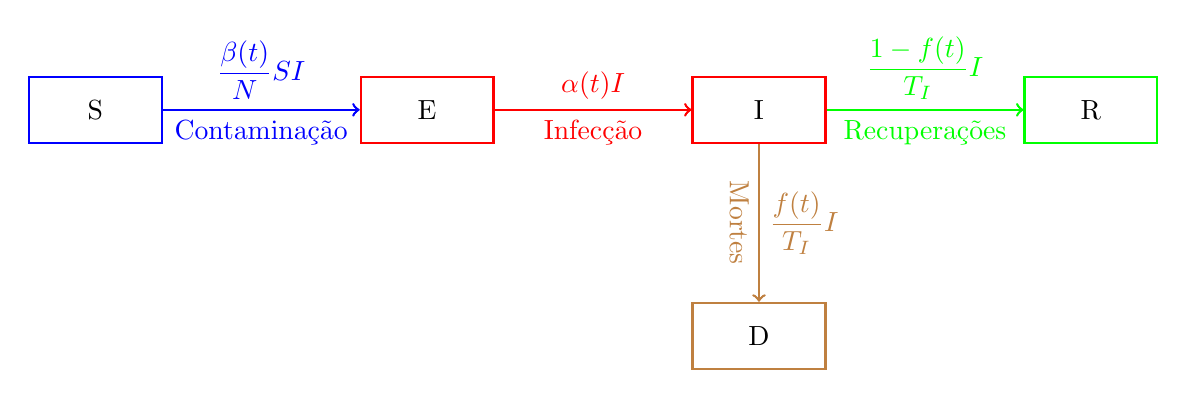
\begin{tikzpicture}[edge from parent/.style = {draw, -latex}]
        \node [entity, draw = blue, thick] (S) {S};
        \node [entity, draw = red, thick] (E) [right = 2.5cm of S] {E};
        \node [entity, draw = red, thick] (I) [right = 2.5cm of E] {I};
        \node [entity, draw = green, thick] (R) [right = 2.5cm of I] {R};
        \node [entity, draw = brown, thick] (D) [below = 2cm of I] {D};
        
        \path[->]
            (S) edge [blue, thick] node[above] {$\dfrac{\beta(t)}{N}SI$} (E)
                edge [blue, thick] node[below] {Contaminação} (E)
            (E) edge [red, thick] node[above] {$\alpha(t) I$} (I)
                edge [red, thick] node[below] {Infecção} (I)
            (I) edge [green, thick] node[above] {$\dfrac{1 - f(t)}{T_I}I$} (R)
                edge [green, thick] node[below] {Recuperações} (R)
                edge [brown, thick] node[right] {$\dfrac{f(t)}{T_I}I$} (D)
                edge [brown, thick] node[sloped, below] {Mortes} (D);
    \end{tikzpicture}
\end{document}